\documentclass[final]{beamer} 
\mode<presentation> {
  \usetheme{Berlin}
}

\usepackage{url}
\usepackage[utf8]{inputenc}
\usepackage{amsmath,amsthm, amssymb, latexsym}
\usefonttheme[onlymath]{serif}
\boldmath
\usepackage[size=custom,width=120,height=80,scale=2,orientation=landscape]{beamerposter}
\title{HLTDI projects}
\author{HLTDI}
\institute[Indiana University]{School of Informatics and Computing, Indiana University}
\date{April 11, 2014}
\begin{document}

\begin{frame}{} 
  \begin{block}
    {\centering \veryHuge Translation for Under-Resourced Languages at IU}\par
    \centering
    {\large Alex Rudnick, Taylor Skidmore, Alberto Samaniego, Annette Rios, and Michael Gasser}
    \par
  \end{block}

\begin{columns}[t]

%%% left column %%% 
  \begin{column}{.33\linewidth}

  \vfill
  %%\begin{block}{\large Contributions}
  \begin{block}{\large Guampa: Collaborative Translation Web Application}
    \centering
    \begin{itemize}
    \item Work together to translate documents!
    \item Comment on and discuss translations to help others learn
    \item Help build the available resources for under-resourced languages
    \item Also helps machine translation researchers build bigger corpora for
    MT system training
    \end{itemize}
  \end{block}

  \begin{block}{\large Guampa Features}
    \centering
    \begin{itemize}
    \item Automatic import of Wikipedia documents: build resources for your 
    \item 
    \item Integrated dictionaries -- 
    \end{itemize}
  \end{block}
  \centering

  \centering
  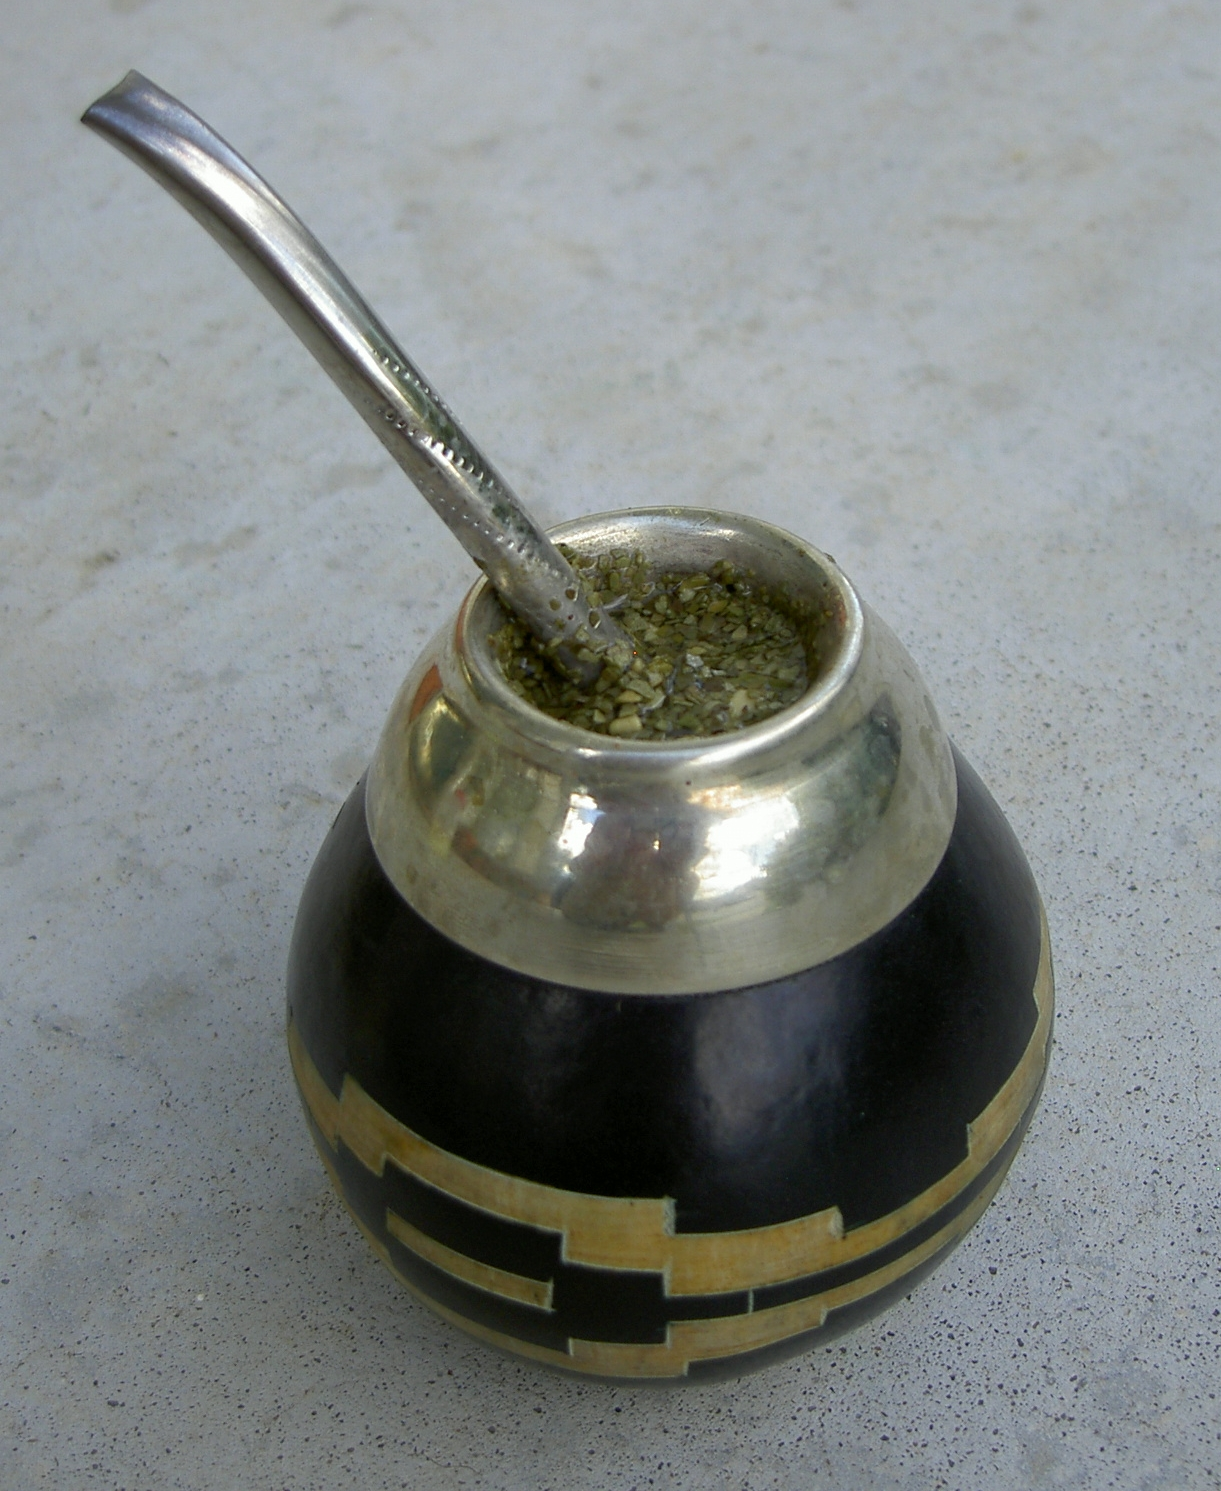
\includegraphics[width=.5\linewidth]{guampa_mate.jpg}
  \end{column}

  %%% middle column %%%
  \begin{column}{.33\linewidth}
  \vfill
  \begin{block}{\large Under-Resourced Languages}
    \begin{itemize}
    \item Roughly 7000 languages in the world; how many do you speak?
    \item Our goal is to support translation into languages with many speakers
    but not lots of data. Current statistical MT approaches are great, but
    don't work well on small data sets.
    \item Focusing on Paraguayan Guarani and Cuzco Quechua
    \end{itemize}
  \end{block}

  \centering
  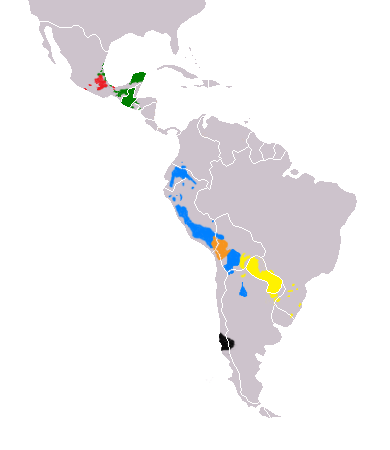
\includegraphics[width=.33\linewidth]{Map-Most_Widely_Spoken_Native_Languages_in_Latin_America.png}
  \begin{block}{Indigenous languages of Latin America}
    \begin{tabular}{lll}
      {\color{blue}    $\blacksquare$} Quechua &
      {\color{yellow}  $\blacksquare$} Guarani &
      {\color{orange}  $\blacksquare$} Aymara \\
      {\color{red}     $\blacksquare$} Nahuatl &
      {\color{green}   $\blacksquare$} Maya languages &
      {\color{black}   $\blacksquare$} Mapudungún
    \end{tabular}
  \end{block}

  \begin{block}{\large Open Source and collaboration}
    \centering
    \begin{itemize}
    \item Working with researchers in the US, Paraguay \& Switzerland
    \item Check out our software!
    \item \url{http://hltdi.github.io}
    \end{itemize}
  \end{block}


  \end{column}

  %% TODO: put some cute pictures: the hula teddy, a chipa, a guampa

  %%% right column %%%
  \begin{column}{.33\linewidth}
  \vfill
  \begin{block}{\large Improving lexical selection}
    \begin{itemize}
    \item Frame picking the right word during translation as a word-sense disambiguation problem
    \item Languages make different distinctions!
    \item Have to learn to distinguish between uses of a source-language word
    that get translated to different target-language words
    \end{itemize}
  \end{block}

  \begin{block}{\large Chipa CL-WSD system}
    \begin{itemize}
    \item We have a lot of good data \& NLP tools for Spanish -- let's use them
    to make better word choices while generating 
    \item Most MT systems 
    \end{itemize}
  \end{block}


  \begin{block}{\large Translation systems}
    \centering
    \begin{itemize}
    \item Chipa integrates with SQUOIA, the Spanish-Quechua MT system from Zürich (see our SALTMIL 2014 paper)
    \item We're working on 
    \item Reusable open source software
    \end{itemize}
  \end{block}
  \hfill
  
\includegraphics[width=.20\linewidth]{hltdi-logo-small.png}


  \end{column}

\end{columns}

\end{frame}
\end{document}
